\documentclass[conference]{IEEEtran}
\usepackage[T1]{fontenc}
\usepackage{amsmath}
\usepackage{amssymb}
\usepackage{booktabs}
\usepackage{graphicx}
\usepackage{array}
\usepackage{microtype}
\usepackage[hidelinks]{hyperref}

\graphicspath{{./}}
\setlength{\emergencystretch}{3em}
\renewcommand{\arraystretch}{1.1}

\begin{document}

\title{Demand Shift Robustness of Learned Fleet Rebalancing on NYC Ride-Hailing Data}

\author{%
\IEEEauthorblockN{Alaa Daoud}
\IEEEauthorblockA{LAMIH, CNRS, INSA Hauts-de-France, UPHF}
\and
\IEEEauthorblockN{Avani Dewangan, Md Athar Sharif, Prashil Thul}
\IEEEauthorblockA{IIIT Naya Raipur, B.Tech CSE 2024--2028}%
}

\maketitle

\begin{abstract}
We measure how much learned zone controllers lose when deployment demand
differs from training demand. Independent (IPPO) and shared-critic (MAPPO)
controllers are trained on one demand distribution on NYC16, a sixteen-zone
network built from real for-hire-vehicle demand in Manhattan, then frozen and
replayed on ten demand shifts, five seeds per algorithm. A greedy dispatcher
and a tuned rolling-horizon linear programme (LP) are the references. Averaged
over the eleven scenarios (the base condition plus ten shifts) all four
policies keep between $91$ and $93\%$ of their base service, so the loss is not
specific to learning. It is concentrated: permuting zone identities costs every
policy $17$ to $22$ points of service, and sending $60\%$ of demand to one zone
costs the learned arms roughly half their service and the LP a third. IPPO and
MAPPO cannot be separated. MAPPO leads by $1.5$ points of service and $41$~km
of empty distance at the base condition, the training rollouts give the
opposite ordering, and across shifts the sign of the gap changes; the one
scenario where IPPO looks ahead needs paired per-seed data to settle. The tuned
LP serves $69.7\%$ of orders at the base condition against $65.2\%$ (MAPPO) and
$63.7\%$ (IPPO) on $290$~km of empty distance against $436$ and $477$~km, and
under shift it is ahead of the learned arms or within a point of them. The
expectation that learning wins in distribution and then loses ground under
shift is not supported: it does not win in distribution against a tuned
baseline.
\end{abstract}

\begin{IEEEkeywords}
fleet rebalancing, multi-agent reinforcement learning, MAPPO, IPPO, dynamic
dispatch, linear programming, demand shift
\end{IEEEkeywords}

\section{Introduction}
\label{sec:intro}

A rebalancing policy is judged on two numbers: the share of orders it serves
and the distance its vehicles drive empty. They trade against each other
almost freely. A vehicle that repositions cannot be dispatched during the move
and the move earns nothing, so spending distance is one way to buy service.
Comparisons drawn at different points on that trade say nothing about which
policy is better, which is why we evaluate the learned arms and both baselines
on the pair rather than on service rate alone.

The problem is demand distribution shift. Ride-hailing demand moves with
seasons, events and new hotspots, and retraining every day is expensive, so
what matters in deployment is how a frozen policy behaves when demand is not
the demand it trained on. We ask three questions on a network built from
recorded demand. RQ1: how much does performance degrade as demand moves away
from the training distribution? RQ2: do IPPO and MAPPO degrade differently under
the same shifts? RQ3: how does their degradation compare with that of a tuned
LP rebalancer? Four outcomes for RQ2 are all publishable: H1, MAPPO is more
robust because its centralised critic learns demand-invariant structure; H2,
IPPO is more robust because the centralised critic overfits training demand; H3,
no meaningful difference; H4, the difference depends on the shift type. The
expectation behind the project, that learning wins in distribution and degrades
under shift, is tested and not assumed.

In short, the loss under shift is modest on average and the same for all four
policies, but it is concentrated in a few shifts (RQ1). IPPO and MAPPO cannot be
told apart at five seeds, with one scenario left open (RQ2). The tuned LP
degrades by about the same share as the learned arms and starts higher, so the
lead that learning was expected to hold in distribution never appears (RQ3).
The learned arms do beat a dispatcher that never relocates by about twenty
points of service, so they do learn to move vehicles; what separates them from
the LP is the empty distance they pay for it. Service rate can be bought with
empty distance, so every comparison below pairs the two.

The evidence is a five-seed shift study on NYC16, a sixteen-zone subnetwork of
Manhattan carrying real FHVHV demand for 2026-04. We train and evaluate each
learned arm on five seeds, so the spread is reported and not a single run, and
both baselines and both algorithms see the same eleven scenarios. We also check
the reward arithmetic against the measured conversion probability of a
relocation. Without that check we could not say whether a poor result came from
the policy or from an incentive that never paid. This is a measurement study:
no new algorithm is proposed, and the base-condition numbers are the reference
for the degradation measurements, not the headline.

Every standard deviation below is the sample standard deviation
(ddof${}=1$), across seeds where the arm is learned and across evaluation
windows where the policy is deterministic. Actions are deterministic argmax
throughout. S0 denotes the base condition on the twelve validation windows and
S6 the same protocol on the twelve test windows; only S6 measures transfer to
demand the models never saw.

\section{Related Work}
\label{sec:related}

Reinforcement learning entered ride-hailing through order dispatch rather than
repositioning. Xu~\emph{et al.}~\cite{xu2018} combine learned value estimates
with combinatorial planning for large-scale dispatch, Lin~\emph{et
al.}~\cite{lin2018} train cooperative agents over a hexagon grid, and
Qin~\emph{et al.}~\cite{qin2020} report a deployed dispatch policy at DiDi.
Those systems decide which vehicle takes which order given the supply already
on the map. Repositioning asks the prior question, where the supply should be
before the order appears, and it is the harder of the two to evaluate because
the cost of a wrong move is invisible in a service-rate table.

Repositioning has its own learning literature. Oda and
Joe-Wong~\cite{oda2018} propose a model-free approach to dynamic fleet
management, Al-Abbasi~\emph{et al.}~\cite{alabbasi2019} distribute the
rebalancing decision across vehicles with deep RL, and Holler~\emph{et
al.}~\cite{holler2019} learn joint dispatching and repositioning. On the
multi-agent side, Li~\emph{et al.}~\cite{li2019} use mean-field MARL for
order dispatching, Shou and Di~\cite{shou2020} study reward design for driver
repositioning, Jiao~\emph{et al.}~\cite{jiao2021} report a real-world
repositioning deployment, and Gammelli~\emph{et al.}~\cite{gammelli2021}
learn rebalancing policies over a graph representation of the network. Our
work differs from all of these in its question: we do not propose a new
rebalancing algorithm, but measure how frozen learned policies degrade under
demand shift relative to a tuned non-learning baseline.

The baseline we use descends from Guo~\emph{et
al.}~\cite{guo2021}, who integrate matching and rebalancing in a
rolling-horizon transportation problem with uncertain demand. Our LP keeps the
transportation structure, adds an exponential moving-average forecast and a
five-minute lookahead, and is tuned on training windows. On the learning side
we use PPO~\cite{schulman2017} in a PettingZoo AEC
environment~\cite{pettingzoo}, with independent critics (IPPO) and a shared
critic (MAPPO) in the form analysed by Yu~\emph{et al.}~\cite{yu2022}. What
we test is whether, at equal evaluation discipline, these algorithms beat a
tuned programme of a different kind.

Because our central question is robustness to distribution shift, we also
position against the generalisation literature. Robust adversarial
RL~\cite{pinto2017} and domain randomisation~\cite{tobin2017} train policies
to be insensitive to environment variation, and Kirk~\emph{et
al.}~\cite{kirk2023} survey zero-shot generalisation in deep RL. Our shift
study is a direct, controlled instance of the generalisation question applied
to fleet rebalancing, and we borrow its evaluation discipline: freeze the
policy, perturb the environment, and report the degradation.

Finally, our credit-assignment design sits in a broader methodological
landscape. Value-decomposition methods such as QMIX~\cite{rashid2018} and
counterfactual baselines such as COMA~\cite{foerster2018} address the
multi-agent credit-assignment problem that our 80/20 reward split handles
heuristically, and MADDPG~\cite{lowe2017} and mean-field
MARL~\cite{yang2018} are the standard centralised-critic alternatives to the
PPO variants we study. We compare only the two PPO variants here; QMIX and
MADDPG are left to future work (Section~\ref{sec:limitations}).

\section{Environment and Protocol}
\label{sec:env}

\subsection{Network, Demand and Fleet}
\label{sec:network}

NYC16 keeps the sixteen taxi zones with the highest for-hire-vehicle volume in
the April 2026 High Volume For-Hire Vehicle trip records published by the New
York City Taxi and Limousine Commission~\cite{tlc_fhvhv_2026} (IDs 68, 79,
112, 145, 161, 162, 163, 164, 170, 230, 231, 234, 236, 237, 246, 249) and
snaps their centroids to a Manhattan road network of 4{,}861 nodes. The study
does not use the whole month: it draws 108 hourly windows from 6--14 April
2026, restricted to the sixteen selected zones. Windows are split by time into
84 for training, 12 for validation and 12 for test; validation and test are
each a single calendar day (13 and 14 April respectively). An episode plays one
window, capped at 130 orders, on 26 vehicles travelling at 30~km/h. Episodes
last 60 minutes in steps of 0.5 minutes, and an order that waits five minutes
cancels. The fleet and order cap fix the pressure at five orders per vehicle
per window and were chosen before any comparison, so a poor result cannot be
blamed on a fleet that was never large enough. We deliberately keep the fleet
small (26 vehicles over 16 zones) so that the credit-assignment and
non-stationarity effects of interest are not swamped by scale; the cost is
that absolute numbers do not transfer to production fleets, which we return to
in Section~\ref{sec:limitations}.

\subsection{Markov Decision Process}
\label{sec:mdp}

We formalise the problem as a cooperative multi-agent Markov decision process
(MDP) $\langle \mathcal{S}, \mathcal{A}, \mathcal{P}, \mathcal{R}, \gamma
\rangle$. The state space $\mathcal{S}$ is the joint observation of the sixteen
zone controllers, described below. The action space $\mathcal{A}$ is the
Cartesian product of sixteen categorical choices, one per zone, each selecting
a destination from the set of legal target zones (33 actions per zone, masked
to the legal relocation destinations at each turn). The transition
$\mathcal{P}$ is the environment dynamics: order arrivals, vehicle movement at
30~km/h, and cancellations after five minutes. The reward $\mathcal{R}$ is the
credit-assigned per-zone signal of Section~\ref{sec:objective}, and $\gamma$
is the discount factor used in PPO training, set to $0.99$.

At each decision step, zone controller $i$ receives a 615-dimensional vector
formed by concatenating nine channels. (i) \emph{zone\_location}
$\in[0,1]^2$: the zone centroid, min--max normalised to the network bounding
box. (ii) \emph{zone\_state} $\in\mathbb{R}^4$: vehicles in $i$ as a share of
the 26-vehicle fleet, the idle fraction within $i$, pending orders in $i$ as a
share of the fleet, and the supply--demand deficit (pending minus idle share).
(iii) \emph{all\_zone\_state} $\in\mathbb{R}^{16\times4}$: the same four
quantities for all sixteen zones. (iv) \emph{pending\_orders}
$\in\mathbb{R}^{16\times6}$: up to sixteen orders whose origin lies in $i$
(nearest centroid, within the 2~km dispatch radius), each described by
normalised origin $(x,y)$, destination $(x,y)$, party size divided by
capacity, and waiting time divided by the timeout; slots are filled
distance-first, then by urgency. (v) \emph{pending\_mask} $\in\{0,1\}^{16}$
marks occupied slots, and (vi) \emph{pending\_passengers}
$\in\mathbb{R}^{16}$ repeats the party-size field. (vii)
\emph{neighbor\_mask} $\in\{0,1\}^{16}$ marks the legal relocation
destinations (the zone's $k$-nearest-centroid neighbours). (viii)
\emph{demand\_hist} $\in\mathbb{R}^{16\times24}$: pending demand in every zone
over the last 24 turns, i.e.\ the last 12 minutes at $\Delta t=0.5$. (ix)
\emph{time\_frac} $\in[0,1]$: the elapsed fraction of the episode. A
sixteenth-dimensional \emph{inbound} channel records the share of the fleet
already travelling toward each zone. Numeric channels are divided by a
per-channel running maximum accumulated within the episode; the observation is
a \texttt{Dict} of \texttt{Box}es, flattened in the above order before
entering the network.

Observations are neither purely local nor fully shared. A controller sees the
detailed order list only for its own zone, but it sees every zone's aggregate
fleet/demand state, every zone's 12-minute demand history, the fleet's inbound
distribution, and its own legal-target mask. There is no demand forecast and no
wall-clock time-of-day feature; the only temporal signals are the 12-minute
history and the elapsed-episode fraction. The MAPPO critic is not fed the
concatenation of the sixteen observations (which would be
$16\times615=9{,}840$ dimensions). It receives the environment's
593-dimensional global state---all-zone fleet state (64), the sixteen most
urgent pending-order feature rows (96), their mask (16), all-zone demand
history (384), the adjacency mask (16), inbound counts (16), and time
(1)---concatenated with the acting zone's own 615-dimensional observation,
$593+615=1{,}208$ dimensions, plus a learned 16-way zone-identity embedding
(256 units) inside the critic.

\subsection{Objective and Credit}
\label{sec:objective}

The team reward trades served orders against the distance and time spent
serving them:
\begin{equation}
  R \;=\; \omega\, n_{\mathrm{served}}
      \;-\; \beta\, d_{\mathrm{empty}}
      \;-\; \alpha\, \bar{w}
      \;-\; c\, n_{\mathrm{cancel}},
  \label{eq:objective}
\end{equation}
with $\alpha=0.2$, $\beta=0.06$, $\omega=1.0$ and $c=1.0$ on NYC16, and
$d_{\mathrm{empty}}$ in kilometres per episode. We write the served-order
weight as $\omega$ to avoid collision with the discount factor $\gamma$ of
Section~\ref{sec:mdp} and the GAE parameter $\lambda$ of
Section~\ref{sec:training-setup}.

Zone controllers share this reward rather than receiving an independent one.
Each zone keeps $80\%$ of the credit and cost it generates and $20\%$ of the
team total, and the relocator share of $0.65$ is split along the relocation
chain so that no zone is charged for a move without receiving part of what the
move produced. The zone rewards sum to \eqref{eq:objective} by construction.
That matters for interpretation: an optimiser maximising the per-zone signal
cannot be paid more than the team objective allows, so a gap to the LP cannot
be explained by a bonus that was added on top of $\omega$.
Table~\ref{tab:params} lists the constants.

\begin{table}[!t]
\centering
\caption{NYC16 configuration. The reward weights are those of
\eqref{eq:objective}.}
\label{tab:params}
\footnotesize
\begin{tabular}{lr}
\toprule
Parameter & Value \\
\midrule
Zones                          & 16 \\
Vehicles                       & 26 \\
Order cap per window           & 130 \\
Episode length / step          & 60 min / 0.5 min \\
Speed                          & 30 km/h \\
Order patience                 & 5 min \\
$\alpha$ (wait)                & 0.2 \\
$\beta$ (empty km)             & 0.06 \\
$\omega$ (served order)        & 1.0 \\
$c$ (cancellation)             & 1.0 \\
Discount factor $\gamma$       & 0.99 \\
Team share of zone reward      & 0.2 \\
Relocator share $s$            & 0.65 \\
PPO: $\epsilon$, entropy, GAE $\lambda$ & 0.2, 0.01, 0.99 \\
PPO: epochs, lr, grad clip     & 4, $3\times10^{-4}$, 0.5 \\
\bottomrule
\end{tabular}
\end{table}

\subsection{Baselines}
\label{sec:baselines}

\textbf{Greedy} assigns each order to the nearest idle vehicle and never
relocates. Its empty distance is pickup travel only, which makes it a floor on
distance rather than a competitive policy on service.

\textbf{LP} is a rolling-horizon transportation programme with an exponential
moving-average demand forecast (smoothing $0.3$), a five-minute lookahead and
a deficit penalty of $1.0$. It solves the matching and rebalancing problem
jointly at every turn. Its hyperparameters were tuned on eight NYC16 training
windows, so it is tuned on the same data the learners were trained on and the
comparison is not handicapped in either direction.

\subsection{Training}
\label{sec:training-setup}

Both algorithms' agents pick a destination from the set of legal target zones,
so the relocation decision is one categorical choice rather than a continuous
displacement. IPPO optimises a separate critic per agent and MAPPO a single
critic over the joint observation. Both use PPO in a PettingZoo AEC
environment, six rollout episodes per iteration, 200 iterations, five seeds
per algorithm. Every reported number is the final iteration. Selecting the
best checkpoint on validation would raise the learned arms by roughly a point
and is not done.

All ten reported runs use the flat MLP encoder (\texttt{arch="mlp"}); the
repository also contains masked-attention encoders, but they were not used for
any result in this paper. The IPPO agent is a single zone actor--critic shared
across all sixteen homogeneous zone controllers: a two-layer trunk
\texttt{Linear(615$\to$256) -- Tanh -- Linear(256$\to$256) -- Tanh}, followed
by two separate linear heads, a 33-way policy head (masked before sampling)
and a scalar value head. Actor and critic therefore share the trunk but not
their output layers. MAPPO uses the same shared actor and adds a separate
centralised critic: \texttt{Linear(1208+256$\to$256) -- Tanh --
Linear(256$\to$256) -- Tanh -- Linear(256$\to$1)}, where the 256 additional
inputs are a learned zone-identity embedding; the critic shares no parameters
with the actor. There are no normalisation or dropout layers; Tanh is the only
activation.

The PPO hyperparameters are identical across algorithms and seeds: discount
factor $\gamma=0.99$, GAE $\lambda=0.99$, Adam learning rate
$3\times10^{-4}$, clip ratio $\epsilon=0.2$, entropy coefficient $0.01$,
value-loss coefficient $0.5$, four PPO epochs per update, four minibatches
(minibatch size 2{,}880 of 11{,}520 transitions), six rollout episodes per
update (720 zone-turns; 11{,}520 agent-transitions), and gradient-norm clip
$0.5$.

\section{Training and Reference Condition}
\label{sec:results}

\subsection{Training}
\label{sec:convergence}

Fig.~\ref{fig:curves} gives the training curves. Service rate rises from about
$60\%$ at iteration~0 to $69$--$70\%$ by iteration~40 and moves by less than a
point over the remaining 160. Empty distance falls from roughly $490$~km to
$450$~km over the same interval, mean wait from $3.2$ to $2.65$ minutes, and
team reward from $-40$ to $+5$. The budget is therefore not what separates the
learned arms from the LP. Whatever the gap is, it survives 160 iterations
without the optimiser closing it.

Two features of the curves matter for RQ2. IPPO holds a marginally higher
service rate than MAPPO for most of training and a marginally lower empty
distance, with the seed bands overlapping throughout. The validation ordering
is the opposite of both (Section~\ref{sec:ippo}). The training KPI is also
about five points above the validation KPI for the same checkpoints. We do not
attribute that gap: training rollouts sample actions on training windows and
validation uses argmax on held-out windows, so the two are different
measurements and only the second is used for any comparison in this paper.

\begin{figure*}[!t]
\centering
\includegraphics[width=0.94\textwidth]{figures/learning_curves.png}
\caption{Training KPIs on NYC16, five seeds per algorithm, 200 iterations.
Thin lines are per-iteration five-seed means, thick lines a nine-iteration
rolling mean of that, and bands are $\pm1$ sample standard deviation across
seeds. Values are on-policy rollouts on training windows, not held-out
validation.}
\label{fig:curves}
\end{figure*}

\subsection{Reference Condition (S0)}
\label{sec:base}

Degradation below is measured against S0, which is also where the baseline is
compared with the learned arms. Table~\ref{tab:s0} gives the S0 numbers and
Fig.~\ref{fig:spread} the per-seed spread. MAPPO serves $20.4$ points more
than greedy and drives $5.9$ times its empty distance; IPPO serves $18.9$
points more at $6.4$ times. The LP serves $24.9$ points more than greedy at
$3.9$ times its distance, and it serves $4.5$ points more than MAPPO at $0.67$
times MAPPO's distance.

\begin{table}[!t]
\centering
\caption{Base-condition (S0) performance on NYC16 validation windows. Learned
arms are five-seed means with sample standard deviations across seeds. The
baselines are deterministic, so their $\pm$ is across evaluation windows. The
last column is the empty distance a policy adds per additional percentage
point of service, measured against greedy. Cancellation rate is
$\mathrm{cancelled}/130$ requests per episode; wait is over completed orders
only.}
\label{tab:s0}
\footnotesize
\resizebox{\columnwidth}{!}{%
\begin{tabular}{lccccc}
\toprule
Method & SR & Empty km & km per $+1$ pp & Cancel & Wait (min) \\
\midrule
LP        & 69.7\% $\pm$ 4.4 & 290 $\pm$ 6  &  8.7 & 16.5\% $\pm$ 3.2 & 2.54 $\pm$ 0.10 \\
MAPPO-200 & 65.2\% $\pm$ 1.2 & 436 $\pm$ 26 & 17.7 & 21.8\% $\pm$ 1.1 & 2.59 $\pm$ 0.15 \\
IPPO-200  & 63.7\% $\pm$ 1.9 & 477 $\pm$ 19 & 21.3 & 23.4\% $\pm$ 2.0 & 2.48 $\pm$ 0.11 \\
Greedy    & 44.8\% $\pm$ 8.4 &  74 $\pm$ 16 &  --  & 43.5\% $\pm$ 6.6 & 2.42 $\pm$ 0.18 \\
\bottomrule
\end{tabular}}
\end{table}

The distance-per-point column sums up the result. Greedy gets its service from pickup travel
alone. The LP pays $8.7$~km for each further point, MAPPO about twice that and
IPPO about two and a half times. Against greedy the learned arms are not worse
off, since they serve $42$ to $46\%$ more orders. Against the LP they are well
behind.

The reward function gives the same ordering. At the 130-order cap, $4.5$
points of service is at most $5.9$ reward units, while the $146$ extra
kilometres MAPPO drives relative to the LP cost $8.8$ units. MAPPO is
therefore about fifteen units per episode behind the LP under its own
objective, before wait and cancellations are counted. We would have distrusted
a result that contradicted the training signal; this one does not.

\begin{figure*}[!t]
\centering
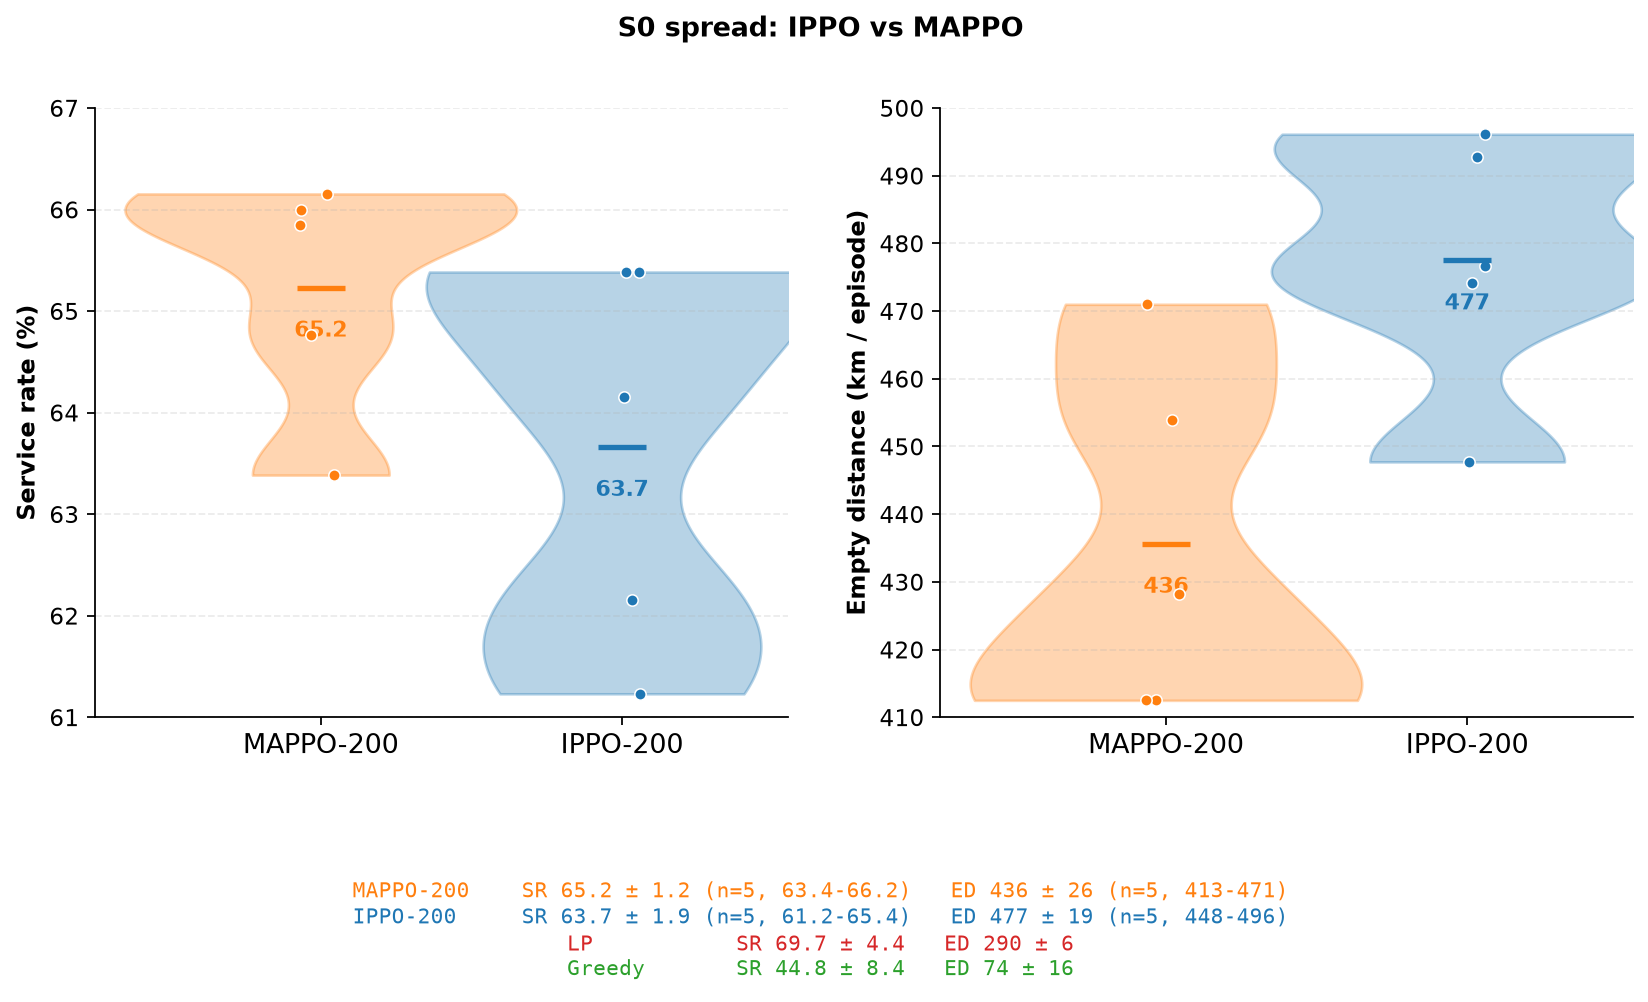
\includegraphics[width=0.85\textwidth]{figures/violin_e_arms_only.png}
\caption{Base-condition spread. Each point is one training seed; the bar is the
five-seed mean. Baselines are deterministic and their spread is across
evaluation windows. Seeds are the unit of replication for the learned arms, so
the width of these distributions is the resolution of every comparison in
Table~\ref{tab:s0}.}
\label{fig:spread}
\end{figure*}

\section{Degradation under Demand Shift}
\label{sec:shifts}

\subsection{Scenarios}
\label{sec:taxonomy}

Each policy is frozen and replayed on ten perturbations of the demand stream.
S1 permutes zone identities spatially, by a rotation offset of half the zone
count, which changes where demand falls without changing how much. S2a, S2b,
S2d and S2e scale the order cap by $0.5$, $0.75$, $1.5$ and $2.0$. S3 replaces
the demand window with a validation-split window. S4 sends $60\%$ of demand to
a single zone (index 1, taxi zone 79). S5 reassigns $20\%$ of orders, in the
interval from minute 20 to minute 30, to a single zone (index 0, taxi zone
68). S6 replays the base protocol on the test split. S7 moves a hotspot from
zone 12 to zone 10 across the episode. Magnitudes are relative to the 130-order
cap, so S2a is 65 orders and S2e is 260.

\subsection{Absolute and Relative Behaviour}
\label{sec:degradation}

Fig.~\ref{fig:panels} gives the absolute service rate, empty distance and wait
under every scenario, and Fig.~\ref{fig:retention} rescales service to each
policy's own S0 so the shapes can be compared directly.

\begin{figure*}[!t]
\centering
\includegraphics[width=0.98\textwidth]{figures/degradation_metrics.png}
\caption{Absolute KPIs under each demand shift, five seeds for the learned arms
and the same evaluation windows for the baselines. Bands are $\pm1$ sample
standard deviation across seeds for the learned arms and across windows for
the baselines. The wait panel is expressed as a change relative to each
policy's own S0 because absolute waits are not comparable across policies that
serve different order mixes.}
\label{fig:panels}
\end{figure*}

Outside S4 no policy falls below $73\%$ of its base service, and the mean
retention across the eleven scenarios lies between $91$ and $93\%$ for all
four. Taken alone, those two facts suggest the shifts do not separate the
policies. They do, and the average hides it.

\begin{figure*}[!t]
\centering
\includegraphics[width=0.98\textwidth]{figures/retention_by_shift.png}
\caption{Service rate under each shift, relative to the same policy's S0. The
vertical axis starts at $45\%$, so bar length is not proportional to
retention; the dashed line is the base condition. Numbers above the S4 bars
give the S4 retention.}
\label{fig:retention}
\end{figure*}

S4 is where the policies separate. Sending $60\%$ of demand to one zone leaves
the LP at $67\%$ of its base service and everyone else at $49$ to $51\%$. In
absolute terms the LP holds $47\%$ where the learned arms fall to $32$ and
$33\%$. This is a concentration shift, not a cold-zone test. Zone 79 carries
$5.99\%$ of training demand against a mean of $6.36\%$, so S4 is a ten-fold
concentration into an ordinary zone that the policies had already seen. The LP
holds up better, which is consistent with its forecast adapting within the
episode, but these runs do not test that explanation.

S2e shows the opposite. When demand doubles (S2e) the LP's relative retention
is the lowest of the four at $73\%$, and its absolute service is $51\%$
against $52\%$ for IPPO. A ranking built on retention alone would call the LP
the least resilient policy in the set; in absolute terms its advantage over
IPPO disappears entirely. The two measures agree everywhere except at doubled
demand, and they disagree there because the LP starts from the highest base.

Smaller shifts behave as the mechanism predicts. Spatial permutation costs
every policy between $17$ and $22$ points, and the LP is no better protected
than greedy, which is consistent with the LP's forecast being a temporal
instrument that does not help when demand moves in space without moving in
time. Under-scaling demand is easier for the baselines than the base condition
($111$ to $114\%$ at S2a, $106$ to $109\%$ at S2b). The learners gain only at
S2b ($107$ to $108\%$) and stay flat at S2a. S5 reassigns existing orders
rather than adding them, into a zone with $6.87\%$ of training demand, so it
is a weak event; it moves no policy by more than two points and does not
discriminate between them.

Empty distance follows the shift rather than the policy. The learned arms
drive about $310$ to $585$~km depending on the scenario, the LP $199$ to
$307$, and greedy $42$ to $110$. At S4 the IPPO arm reaches about $585$~km,
close to its S2a value, while MAPPO stays near $420$~km. The seed band for
IPPO at S4 spans roughly $400$ to $660$~km, so we do not read that $165$~km
gap as an algorithm difference; it is the same instability that makes the
algorithm comparison inconclusive at S0.

\subsection{Held-out Demand}
\label{sec:heldout}

S6 is the only non-synthetic scenario and the only one drawn from windows no
model saw. Retention there is $99$ to $105\%$, and absolute service is about
$67\%$ for both learned arms against $69\%$ for the LP, so the ranking of
Section~\ref{sec:base} does not depend on the validation split. S6 rules out a
split artefact: the validation windows did not produce the ordering. It shows
no benefit from unfamiliar demand either, since both learned arms just
reproduce their base service and distance.

\subsection{IPPO against MAPPO (RQ2)}
\label{sec:ippo}

At S0 MAPPO is ahead by $1.5$ points of service and $41$~km of empty distance,
and looks better on both axes at once, but five seeds do not resolve either
difference. Across the five seeds MAPPO's service rate runs from $63.4$ to
$66.2\%$ and IPPO's from $61.2$ to $65.4\%$; empty distance runs from $413$ to
$471$~km for MAPPO and $448$ to $496$~km for IPPO, so the ranges overlap on
both axes. The training curves of Fig.~\ref{fig:curves} put IPPO ahead on both
axes for the second half of training. Since two measurement streams disagree
on the sign of both differences, we do not attribute the S0 ordering to the
shared critic.

Under shift the two arms move together (Fig.~\ref{fig:retention}). Read off
the figure, their retention differs by under two points in S1, S5 and S7, by
two to three points in S2a, S2d, S2e, S4 and S6, and by about seven points in
S3. IPPO retains more at S2d, S2e, S3 and S6, MAPPO at S2a and S4. S3 is the
only gap large enough to look like an effect: IPPO's absolute service there is
about $68\%$ against about $65\%$ for MAPPO, more than the S0 seed standard
deviations of $1.9$ and $1.2$ points. A paired per-seed comparison on identical
windows would settle it. We cannot run that comparison from the retained
figures, so S3 is reported as unresolved and not as support for H2.

\subsection{Answer to H1--H4}
\label{sec:hypotheses}

H1 and H2 are not supported as general statements: the sign of the retention
gap changes between scenarios and mean retention sits in the same $91$ to
$93\%$ band for both arms. H3 describes S0 and every shift except S3. H4 is
not excluded, since S3, the temporal shift implemented as a different set of
windows, is the one scenario where IPPO is ahead by more than the S0 seed
spread, but one scenario is not a pattern. The expectation that learning wins
in distribution and degrades under shift fails at its first half, because the
tuned LP is ahead of both learned arms at S0 and ahead or within a point of
them under every shift. The second half holds but is not specific to learning:
every policy loses most under spatial permutation and concentration.

\section{Relocation Economics}
\label{sec:economics}

A relocation costs $\beta L$, where $L$ is the leg plus the pickup deadhead it
induces. Measured on NYC16 validation, $L=2.9+1.46=4.36$~km, so a move costs
$0.06\times4.36=0.262$ reward units. It earns $s\omega=0.65$ only if the
moved vehicle is dispatched and completes. The break-even conversion
probability is therefore
\begin{equation}
  p \;>\; \frac{\beta L}{s\omega}
      \;=\; \frac{0.06\times4.36}{0.65\times1.0}
      \;=\; 0.40 .
  \label{eq:breakeven}
\end{equation}
Measured conversion is $0.568$ for a move into a zone with unmet demand and
$0.329$ for a move into an empty zone. The threshold sits between the two, so
the incentive is well posed: a policy that aims at need clears it, and a
policy that aims at nothing does not.

The margin is thin. A perfectly aimed move nets $0.108$ units and a wasted
move loses $0.048$, a spread of $0.156$ per decision against a return whose
scale is set by tens of served orders per episode. A difference of that size
is learnable in principle and slow in practice, and it is the reason we expect
destination choice to be the last part of the policy to sharpen. We did not
measure targeting directly on these checkpoints, so that remains an inference
rather than a result.

Two things follow. The incentive is not broken, so the gap to the LP is not an
artefact of a reward that made relocation unprofitable. It is not generous
either, so the learned arms' $436$ to $477$~km fits a policy that finds moving
easy to justify and aiming hard to learn.

\section{Limitations}
\label{sec:limitations}

The study covers one network, sixteen zones of Manhattan, and 108 hourly
windows drawn from 6--14 April 2026---not the full month. Sixteen zones with
twenty-six vehicles is smaller than any deployment, and the LP's advantage may
shrink or grow with zone count; nothing here establishes which. The
constant-speed assumption (30~km/h with no congestion and no time-varying
travel times) is a simplification that affects the empty-distance metric
directly, and we do not test its sensitivity. Validation and test are each a
single calendar day, so the transfer measurement of S6 rests on one day of
demand.

Five seeds resolve the distance gap but not the service gap. The LP's service
advantage over MAPPO is $4.5$ points with overlapping bands, so the defensible
claim is about the pair of criteria, where the LP dominates, rather than about
service rate alone.

Absolute wait is not part of the evaluation summary, so wait is reported only
as a change relative to each policy's own base. A policy that serves a
different order mix can therefore show a smaller wait change without serving
anyone faster, and we do not use the wait panel to rank the policies.

Each algorithm was trained at a single hyperparameter setting---$\beta=0.06$
and an $80/20$ team split with a $0.65$ relocator share---and not tuned
against the LP's tuning budget, so the learned arms might improve. Neither the
empty-distance penalty nor the credit split was swept, so the headline
exchange rate (roughly twice the LP's empty distance per point of service) is
conditional on $\beta=0.06$ and untested at other values. The LP was tuned on
training windows rather than on validation or test, so its edge does not come
from tuning on the evaluation set. We compare only two learned algorithms
(IPPO and MAPPO) against greedy and LP; value-decomposition (QMIX) and
continuous-action (MADDPG) baselines are left to future work.

S4 is not a cold-zone test. The sixteen busiest zones were selected by
training volume, so none is cold: the coldest carries $4.84\%$ of training
demand against a mean of $6.36\%$, a spread of $1.7\times$. Whether a policy
copes with demand in a zone it never saw is therefore not tested here, and S1
is the closest scenario we have. An earlier version of this draft called S4 a
cold-zone result; that label was wrong on this build.

Finally, S0 is a validation split and S6 the only transfer measurement. One
scenario (S5) moves no policy by more than two points and one (S6) is a replay
rather than a perturbation, so the eleven labels overstate the range of
behaviour actually tested.

\section{Conclusion}
\label{sec:conclusion}

We asked how much frozen zone controllers lose when demand moves away from
their training distribution, whether IPPO and MAPPO lose differently, and how
that compares with a tuned LP. On NYC16 the loss is modest on average and
shared by all four policies, it is concentrated in spatial permutation and in
concentration of demand into one zone, IPPO and MAPPO are not separable at
five seeds, and the tuned LP is ahead of both at S0 and ahead or within a
point of them under shift. The learned policies raise greedy's service rate by
$42$ to $46\%$ and pay about six times its deadhead for it, so we do not call
them failures. The LP serves more orders than either at $0.61$ to $0.67$ of
their distance, so we do not call them winners.

The number worth remembering is the exchange rate. The LP needs $8.7$~km of
empty travel per point of service, MAPPO $17.7$ and IPPO $21.3$. A learned
policy that closed that gap would have to convert distance into service at the
LP's rate, and nothing in the training curves suggests the 200-iteration
budget is what prevents it.

Under shift the policies are closer than their base numbers suggest. All four
retain about the same share of service on average, and the LP's lead is widest
when $60\%$ of demand goes to one zone, where it loses a third of its service
and the learned arms lose half. These runs do not say why. At doubled demand
the absolute gap shrinks to a point and the relative ranking flips, because
retention depends on the base as much as on the policy.

\section*{Reproducibility}
\begingroup
\raggedright

Code and figures: \url{https://github.com/sharifmdathar/marl-fleet-rebalancing}.
Training and evaluation are driven by
\texttt{python -m} \path{marl_fleet_rebalancing.experiments.train} and
\texttt{python -m} \path{marl_fleet_rebalancing.experiments.evaluate} with
\texttt{-{}-env nyc}.

\begin{sloppypar}
The checkpoints and raw evaluation outputs behind every table are packaged in
a versioned archive (49~MB, SHA-256
\texttt{3c3f9500d26738d9}\allowbreak\texttt{9085a3dd3cb1dd47}\allowbreak
\texttt{cc94252bcdd37519}\allowbreak\texttt{15aeb056c0c2bfb2}), available
from the authors on request; with it the tabulated values are re-evaluable
exactly, though bit-exact retraining is not established. Full setup, data
download, per-script usage, and the archive contents are documented in the
repository README.
\end{sloppypar}

\par
\endgroup

\begin{thebibliography}{1}
\bibitem{guo2021} X. Guo, N. S. Caros, and J. Zhao, ``Robust
matching-integrated vehicle rebalancing in ride-hailing system with uncertain
demand,'' \emph{Transportation Research Part B: Methodological}, vol. 150,
2021.
\bibitem{pettingzoo} J. K. Terry \emph{et al.}, ``PettingZoo: Gym for
multi-agent reinforcement learning,'' in \emph{Proc. NeurIPS}, 2021.
arXiv:2009.14471.
\bibitem{xu2018} Z. Xu \emph{et al.}, ``Large-scale order dispatch in
on-demand ride-hailing platforms: A learning and planning approach,'' in
\emph{Proc. ACM SIGKDD}, 2018.
\bibitem{lin2018} K. Lin, R. Zhao, Z. Xu, and J. Zhou, ``Efficient large-scale
fleet management via multi-agent deep reinforcement learning,'' in
\emph{Proc. ACM SIGKDD}, 2018.
\bibitem{qin2020} Z. T. Qin \emph{et al.}, ``Ride-hailing order dispatching at
DiDi via reinforcement learning,'' \emph{INFORMS Journal on Applied
Analytics}, vol. 50, no. 5, 2020.
\bibitem{schulman2017} J. Schulman, F. Wolski, P. Dhariwal, A. Radford, and O.
Klimov, ``Proximal policy optimization algorithms,'' arXiv:1707.06347, 2017.
\bibitem{yu2022} C. Yu, A. Velu, E. Vinitsky, J. Gao, Y. Wang, A. Bayen, and
Y. Wu, ``The surprising effectiveness of PPO in cooperative multi-agent
games,'' in \emph{Proc. NeurIPS}, 2022.
\bibitem{oda2018} T. Oda and C. Joe-Wong, ``MOVI: A model-free approach to
dynamic fleet management,'' in \emph{Proc. IEEE INFOCOM}, 2018.
\bibitem{alabbasi2019} A. O. Al-Abbasi, A. Ghosh, and V. Aggarwal, ``DeepPool:
Distributed model-free algorithm for ride-sharing using deep reinforcement
learning,'' \emph{IEEE Transactions on Intelligent Transportation Systems},
vol. 20, no. 12, 2019.
\bibitem{holler2019} J. Holler, R. Vuorio, Z. Qin, X. Tang, Y. Jiao, T. Jin,
S. Singh, C. Wang, and J. Ye, ``Deep reinforcement learning for multi-driver
vehicle dispatching and repositioning problem,'' in \emph{Proc. IEEE ICDM},
2019.
\bibitem{li2019} M. Li, Z. Qin, Y. Jiao, Y. Yang, J. Wang, C. Wang, G. Wu,
and J. Ye, ``Efficient ridesharing order dispatching with mean field
multi-agent reinforcement learning,'' in \emph{Proc. WWW}, 2019.
\bibitem{shou2020} Z. Shou and X. Di, ``Reward design for driver
repositioning using multi-agent reinforcement learning,'' \emph{Transportation
Research Part C: Emerging Technologies}, vol. 119, 2020.
\bibitem{jiao2021} Y. Jiao, X. Tang, Z. Qin, S. Li, F. Zhang, H. Zhu, and J.
Ye, ``Real-world ride-hailing vehicle repositioning using deep reinforcement
learning,'' \emph{Transportation Research Part C: Emerging Technologies},
vol. 130, 2021.
\bibitem{gammelli2021} D. Gammelli, K. Yang, J. Harrison, F. Rodrigues, F. C.
Pereira, and M. Pavone, ``Graph neural network reinforcement learning for
autonomous mobility-on-demand systems,'' in \emph{Proc. IEEE CDC}, 2021.
\bibitem{pinto2017} L. Pinto, J. Davidson, R. Sukthankar, and A. Gupta,
``Robust adversarial reinforcement learning,'' in \emph{Proc. ICML}, 2017.
\bibitem{tobin2017} J. Tobin, R. Fong, A. Ray, J. Schneider, W. Zaremba, and
P. Abbeel, ``Domain randomization for transferring deep neural networks from
simulation to the real world,'' in \emph{Proc. IEEE/RSJ IROS}, 2017.
\bibitem{kirk2023} R. Kirk, A. Zhang, E. Grefenstette, and T. Rockt\"aschel,
``A survey of generalisation in deep reinforcement learning,'' \emph{Journal
of Artificial Intelligence Research}, vol. 77, 2023.
\bibitem{rashid2018} T. Rashid, M. Samvelyan, C. Schroeder de Witt, G.
Farquhar, J. Foerster, and S. Whiteson, ``QMIX: Monotonic value function
factorisation for deep multi-agent reinforcement learning,'' in \emph{Proc.
ICML}, 2018.
\bibitem{foerster2018} J. Foerster, G. Farquhar, T. Afouras, N. Nardelli, and
S. Whiteson, ``Counterfactual multi-agent policy gradients,'' in \emph{Proc.
AAAI}, 2018.
\bibitem{lowe2017} R. Lowe, Y. Wu, A. Tamar, J. Harb, P. Abbeel, and I.
Mordatch, ``Multi-agent actor-critic for mixed cooperative-competitive
environments,'' in \emph{Proc. NeurIPS}, 2017.
\bibitem{yang2018} Y. Yang, R. Luo, M. Li, M. Zhou, W. Zhang, and J. Wang,
``Mean field multi-agent reinforcement learning,'' in \emph{Proc. ICML}, 2018.
\bibitem{tlc_fhvhv_2026} New York City Taxi and Limousine Commission.
\newblock High Volume For-Hire Vehicle Trip Records, April 2026 [data set].
\newblock NYC TLC Trip Record Data, 2026.
\newblock \url{https://www.nyc.gov/site/tlc/about/tlc-trip-record-data.page}
  (file: \texttt{fhvhv\_tripdata\_2026-04.parquet}).
\newblock Accessed 5 November 2026.
\end{thebibliography}

\end{document}